\chapter{Progettazione concettuale}
    \section{Class Diagram}
    
    \begin{figure}[htbp]
    \begin{center}
        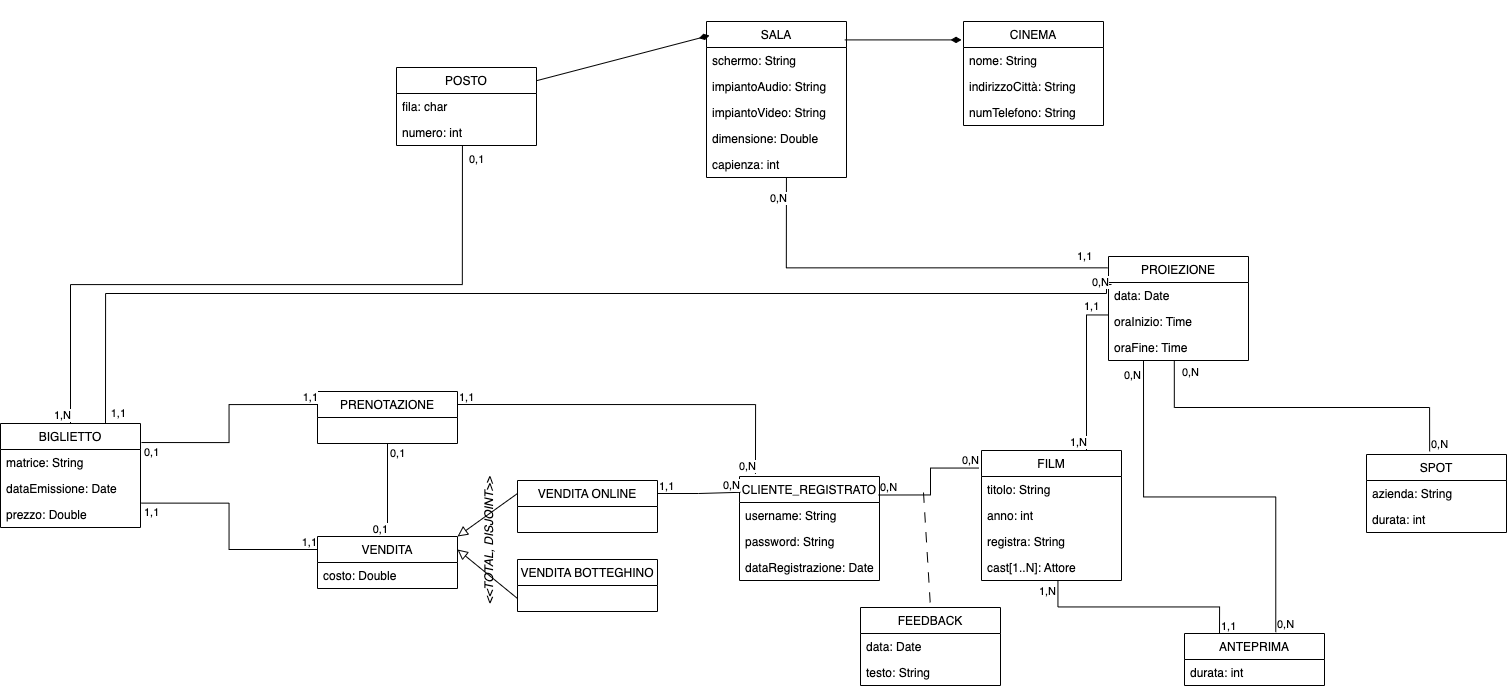
\includegraphics[width=12cm]{Immagini/Schema ER.png}
    \end{center}
    \end{figure}
    \section{Analisi della ristrutturazione del Class Diagram}
        In questa fase ci occupiamo di rendere il Class Diagram idoneo alla traduzione in schemi relazionali, in particolare verranno rimosse:
        \begin{itemize}
            \item Le Generalizzazioni e Specializzazioni
            \item Gli attributi multipli
            \item Gli attributi strutturati
        \end{itemize}
        
        
        
        \subsection{Analisi delle ridondanze}
                \label{analisireq}
            L'unica ridondanza che abbiamo ritenuto fosse il caso di rimuovere è l'entità \textbf{Vendita} che ha come unico attributo \textit{costo}, anche presente nell'entità \textbf{Biglietto}.
            
            
        \subsection{Analisi degli identificativi}
            Nell'analisi degli identificativi provvederemo a scegliere uno o più attributi che garantiranno il rispetto dell'integrità referenziale per ogni tupla.
            
            In particolare notiamo che:
 \begin{itemize}
 
 
     \item \textbf{Cinema}: si è scelto di aggiungere un attributo \underline{ID\_Cinema} e renderlo chiave primaria.
     
     \item \textbf{Sala}: è già presente un attributo \underline{Numero} che rappresenta una potenziale chiave primaria insieme alla chiave esterna \underline{\textit{ID\_Cinema}}.
     
     \item \textbf{Posto}: sono già presenti degli attributi \underline{Fila} e \underline{Numero} che insieme alle chiavi esterne \textit{Cinema} e \textit{Sala} permettono di identificare univocamente ogni poltrona.
     \footnote{\textit{Sarebbe utile creare un attributo ID\_Poltrona?}}
    
     
     \item \textbf{Proiezione}: si è scelto di aggiungere un attributo \underline{ID\_Proiezione} così da non dover utilizzare una chiave primaria composta da tutti gli attributi dell'entità.
     
     \item \textbf{Film}: si è scelto di aggiungere un attributo \underline{ID\_Film} e renderlo chiave primaria.
     
     \item \textbf{Trailer}: si è scelto di aggiungere un attributo \underline{ID\_Trailer} per identificare univocamente i singoli trailer.
     
     \item \textbf{Spot}: abbiamo ritenuto che il nome di un'azienda non fosse abbastanza per identificare una pubblicità, è stato quindi aggiunto un attributo \underline{ID\_Spot} ed è stato reso chiave primaria.
     
     \item \textbf{Biglietto}: si è scelto di modificare il nome dell'attributo \textit{matrice} e farlo diventare \underline{ID\_Biglietto} e di rendere lo stesso chiave primaria.
     
     \item \textbf{Cliente}: è già presente un attributo \underline{Username} che rappresenta una potenziale chiave primaria.
     
     \item \textbf{Recensione}: è stato aggiunto un attributo \underline{ID\_Recensione} per identificare univocamente le recensioni. 
     
     
 \end{itemize}
 
 
 
        \subsection{Rimozione degli attributi multipli}
            In questa sezione ci occuperemo di rimuovere eventuali attributi multivalore:
            
            In questo Class Diagram è presente un solo attributo multivalore:
            
            \begin{itemize}
                \item \textit{Attori}, all'interno dell'entità \textbf{Film} che abbiamo provveduto a trasformare in una entità a sé stante avente come attributi \underline{Nome}, \underline{Cognome} e \underline{Data di nascita}.
            \end{itemize}
            
            
            
        \subsection{Rimozione degli attributi composti}
        
        In questo Class Diagram non sono presenti attributi composti.
        
            
        \subsection{Partizione/Accorpamento delle associazioni}
        Non si è ritenuto necessario effettuare alcun accorpamento di entità.
            
        
        
        \subsection{Rimozione delle gerarchie}
    
    L'unica generalizzazione presente era
        \textbf{Vendita}, che aveva come entità figlie Vendita Online e Vendita Botteghino, che sono state rimosse nel punto \ref{analisireq} e sostituite dall'attributo \textit{Modalita\_Acquisto} di tipo MOD\_ACQUISTO inserito come enumerazione nell'entità \textbf{Biglietto}.
        
    
    \section{Class Diagram ristrutturato}
    \begin{figure}[htbp]
    \begin{center}
        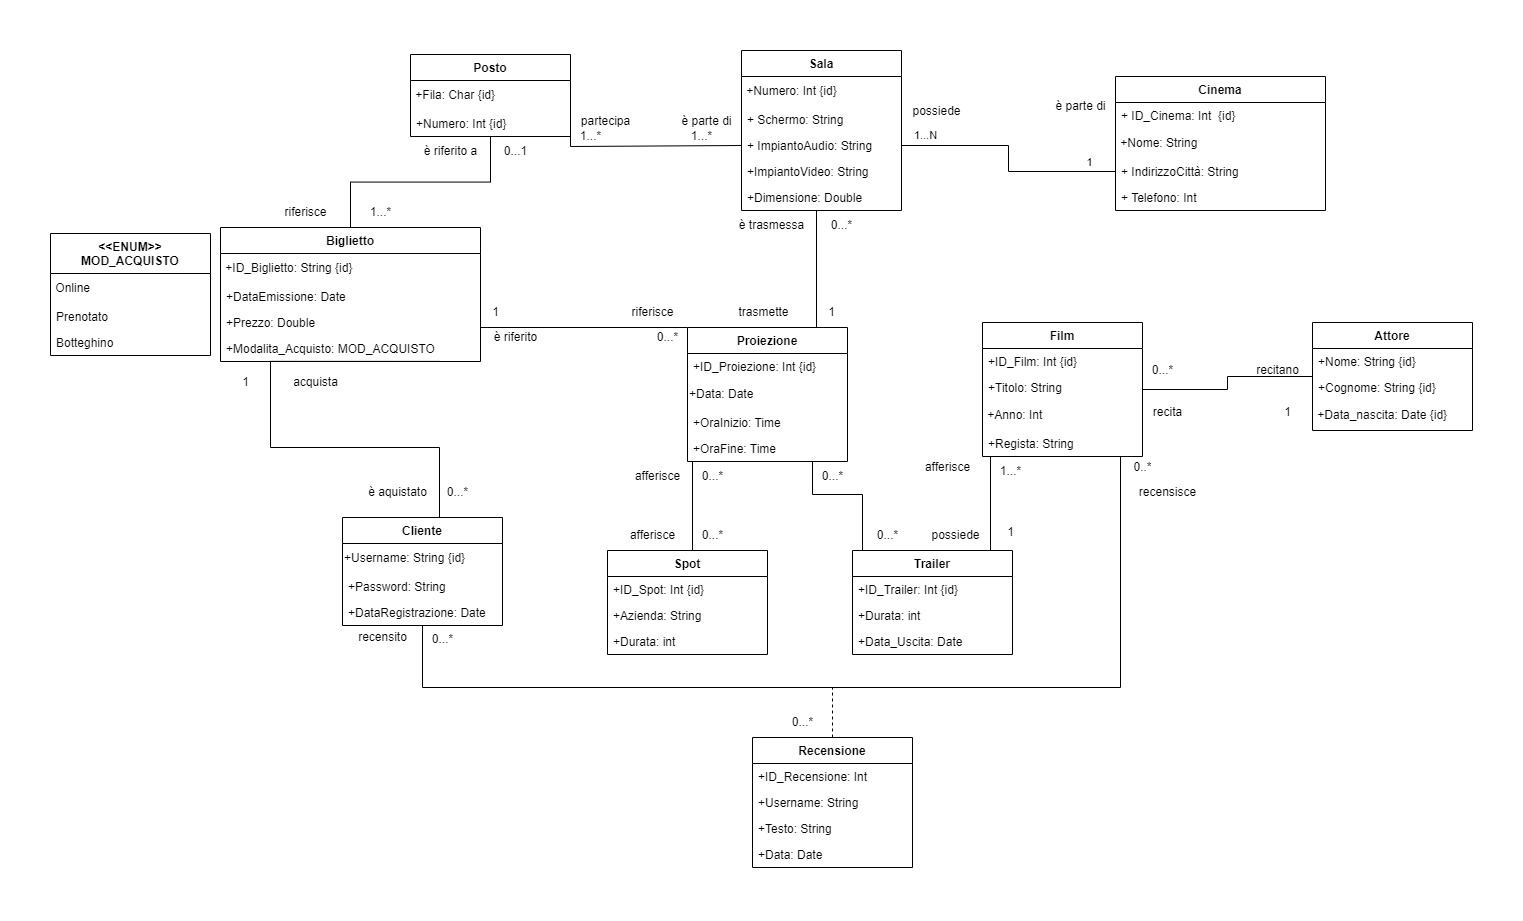
\includegraphics[width=12.1cm]{Immagini/CD Ristrutturato final.jpg}
    \end{center}
    \end{figure}
    
        
    \section{Dizionario delle classi}
        
    \section{Dizionario delle associazioni}